\documentclass[11pt]{article}

\usepackage[margin=1in]{geometry}
\usepackage{booktabs}
\usepackage{enumitem}
\usepackage{tikz}
\usetikzlibrary{arrows.meta, positioning}
\usepackage[hidelinks]{hyperref}

\newcommand{\code}[1]{\texttt{#1}}

\tikzset{
  box/.style={draw, rounded corners, minimum height=0.8cm, align=center, font=\small},
  arrow/.style={-{Stealth}, thick},
  subscription/.style={-{Stealth}, thick, dashed},
  lbl/.style={font=\footnotesize, midway, above},
}

\title{PatchCore Feedback: Why Not One Flow}
\author{Design note}
\date{\today}

\begin{document}
\maketitle

\section{Summary}

PatchCore learns from a remote verifier: when the verifier says a suspected
anomaly was a false positive, PatchCore adds that frame's features to its
memory bank. This note compares two ways to deliver the verifier's verdicts to
PatchCore's updater, and explains why putting the updater at the end of the
detection flow is a poor choice, \emph{even if} the design allowed input edges
from remote to local engines.

\textbf{Recommendation:} keep the detection flow as
\code{camera} $\to$ \code{patchcore-score} $\to$ \code{verifier}, and let
\code{patchcore-update} \emph{subscribe} to the verifier's event service. Making
the updater part of the flow ties PatchCore's frame rate to the speed of its
memory-bank updates, can stop scoring entirely for the length of an update,
drops verdicts that the cloudlet already computed, and needs a new kind of
edge for a single use case.

\section{The two designs}

In both designs, PatchCore runs as one process with two engine endpoints,
sharing the memory bank:
\begin{itemize}[nosep]
  \item \code{patchcore-score} scores frames against the memory bank;
  \item \code{patchcore-update} updates the memory bank from verdicts, on its
        own thread, and the score thread swaps the new bank in between frames.
\end{itemize}

\begin{figure}[h]
\centering
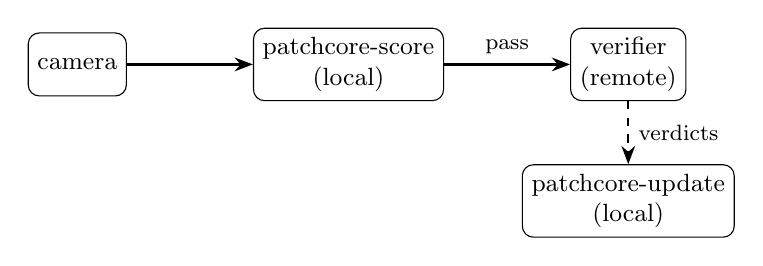
\begin{tikzpicture}[node distance=0.8cm and 1.6cm]
  \node[box] (cam) {camera};
  \node[box, right=of cam] (score) {patchcore-score\\(local)};
  \node[box, right=of score] (ver) {verifier\\(remote)};
  \node[box, below=of ver] (upd) {patchcore-update\\(local)};
  \draw[arrow] (cam) -- (score);
  \draw[arrow] (score) -- node[lbl] {pass} (ver);
  \draw[subscription] (ver) -- node[font=\footnotesize, midway, right] {verdicts} (upd);
\end{tikzpicture}

\vspace{0.4cm}
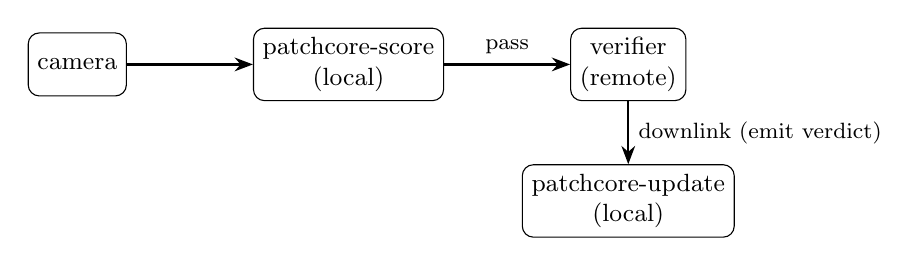
\begin{tikzpicture}[node distance=0.8cm and 1.6cm]
  \node[box] (cam) {camera};
  \node[box, right=of cam] (score) {patchcore-score\\(local)};
  \node[box, right=of score] (ver) {verifier\\(remote)};
  \node[box, below=of ver] (upd) {patchcore-update\\(local)};
  \draw[arrow] (cam) -- (score);
  \draw[arrow] (score) -- node[lbl] {pass} (ver);
  \draw[arrow] (ver) -- node[font=\footnotesize, midway, right] {downlink (emit verdict)} (upd);
\end{tikzpicture}
\caption{Top: the recommended design. The flow ends at the verifier, and the
updater subscribes to the verifier's events (dashed). Bottom: the single-flow
design. The verifier emits its verdict as a new input, which travels back to
the device on a remote-to-local edge.}
\label{fig:designs}
\end{figure}

\paragraph{Subscription (recommended).} The flow ends at the verifier. The
verifier reports its verdict as an ordinary result. The client republishes the
verifier's events on the device, and \code{patchcore-update} reads every
verdict from its subscription.

\paragraph{Single flow.} The flow continues from the verifier to
\code{patchcore-update}. This needs the design extended in two ways: an input
edge from a remote engine to a local one (a \emph{downlink}), owned by the
client, and a verifier that \code{Emit}s its verdict as a new input, so that
the small verdict, not the frame, travels back.

\section{Why the single flow is a poor choice}

\subsection{The frame rate depends on the updater}

Tokens are end-to-end: an input keeps its token until its path completes. In
the single flow, the path of a suspected anomaly ends at the updater, so its
token is held through the verifier \emph{and} the memory-bank update. A
verdict waiting in the updater's pending slot also holds its token. Normal
frames are not affected: they complete at \code{patchcore-score}.

So the more anomalies the scene has, and the slower the update, the fewer
tokens are left for scoring. PatchCore's anomaly detection slows down
\emph{because} its memory bank is slow to train. With a subscription, an
anomaly's token returns as soon as the verifier finishes, and the update never
affects the frame rate.

\subsection{Scoring can stop entirely}

Take two tokens, scoring at 0.05~s per frame, verification at 0.3~s including
the network, and a memory-bank rebuild of 2~s:
\begin{enumerate}[nosep]
  \item Anomaly A is verified as a false positive, and the updater starts a
        2~s rebuild. A's token stays held.
  \item Anomaly B is verified next. The updater is busy, so B's verdict waits in
        the updater's pending slot, and B's token stays held too.
  \item Both tokens are held, so no new frame can be admitted, and
        \code{patchcore-score} sits idle.
  \item B's verdict would be released if a newer verdict replaced it, but no
        new verdict can come, because no frame can be admitted to produce one.
\end{enumerate}
Scoring therefore stops until A's rebuild finishes: up to 2~s with no anomaly
detection at all, every time two anomalies arrive close together. More tokens
only move the threshold: with $C$ tokens, $C$ anomalies in a row stop scoring.
With a subscription, both tokens return after verification, and scoring
continues throughout.

\subsection{Verdicts are dropped after the work is done}

In a flow, a busy engine's pending slot keeps only the newest input. With a
slow updater, older verdicts are replaced and dropped. But each dropped verdict
was already computed by the cloudlet and sent back over the network: the
expensive part is done, and only the cheap part is skipped. For a memory bank,
every false positive is useful training signal, so dropping verdicts discards
exactly what the feedback loop is for. Newest-wins exists to avoid sending
stale frames; for verdicts, which are small and already paid for, it is the
wrong policy.

With a subscription, the updater receives every verdict, in order, and can
decide itself how to batch or merge them into its next rebuild.

\subsection{The verifier's code depends on the flow}

In the single flow, the verifier must \code{Emit} its verdict as a new input
for the updater, while the app still wants the verdict as an ordinary result.
So the verifier must report both, and behave differently depending on whether
anything follows it in the flow. Engines are meant to decide \emph{what} to
forward, never \emph{where}, so that the same engine works in any flow. With a
subscription, the verifier always just reports its verdict as a result, and
any number of consumers, the updater, the app, or a monitoring tool, read it.

\subsection{Downlinks are a new mechanism for one use case}

The design today moves inputs only from the device to the cloudlet; results
come back as events. Remote-to-local input edges would add:
\begin{itemize}[nosep]
  \item emitted inputs carried back inside result events, and forwarded by the
        client to the local server;
  \item a new edge kind for the flow compiler, the ownership rules, and the
        install protocol;
  \item new failure cases, such as a disconnection while a verdict is on its
        way back, which ends offers on both sides of the link;
  \item a second direction of input traffic on a link that may be weak.
\end{itemize}
Every one of these must be built, tested, and maintained, to deliver what the
event services already deliver.

\subsection{Deadlines must cover the update}

A ticket's deadline is a backstop for an input stuck anywhere on its path. In
the single flow, the path includes the update, so the deadline must exceed the
verifier's time plus a full rebuild. That either makes the backstop too slow
to catch real failures in scoring and verification, or, if set short, returns
tokens while updates are still running and reports them as timed out.

\section{Comparison}

\begin{center}
\small
\begin{tabular}{@{}p{0.3\linewidth}p{0.3\linewidth}p{0.3\linewidth}@{}}
\toprule
& Subscription & Single flow \\
\midrule
Anomaly's token held until & the verifier finishes & the update finishes \\
Slow updates affect scoring & no & yes; scoring can stop \\
Verdicts delivered & every one, in order & newest only, while busy \\
Verifier code & always reports a result & must also emit for the updater \\
New mechanisms needed & none & downlink edges \\
Bounding the update work & the updater batches verdicts & tokens and the pending slot \\
\bottomrule
\end{tabular}
\end{center}

\section{When a single flow would be reasonable}

If an update were as fast as scoring, e.g.\ an incremental append to the
memory bank taking milliseconds, the token coupling would be negligible. Even
then, the single flow would still need downlink edges and an emitting
verifier, and would still drop verdicts. The subscription is simpler in every
case, so it is the design to use.

\end{document}
